\documentclass[aspectratio=169,11pt]{beamer}

\usetheme{Madrid}
\usecolortheme{default}
\setbeamertemplate{navigation symbols}{}
\setbeamertemplate{footline}[frame number]

\usepackage{booktabs}
\usepackage{graphicx}
\usepackage{tabularx}
\usepackage{array}

\title{Prompt and Format Robustness in LLM Evaluation}
\author{Allen Ma}
\institute{
M.S. Computer Science, UCLA\\
Capstone Advisor: Kai-Wei Chang
}
\date{}

\newcommand{\smallgap}{\vspace{0.35em}}

\begin{document}

\begin{frame}
  \titlepage
\end{frame}

\begin{frame}{Motivation}
  \begin{itemize}
    \item LLM evaluations often report one score from one prompt template.
    \item Prior work shows that seemingly minor prompt-format choices can move measured performance.
    \item This creates an evaluation problem: a reported score may partly reflect prompt choice, not just model ability.
  \end{itemize}

  \smallgap
  \begin{block}{Core idea}
    Hold the task examples and model fixed, vary only the prompt wrapper and output-format constraint, then measure how much the score changes.
  \end{block}
\end{frame}

\begin{frame}{Literature Framing}
  \begin{tabularx}{\linewidth}{>{\raggedright\arraybackslash}p{0.22\linewidth} X}
    \toprule
    Paper & Role in this project \\
    \midrule
    Sclar et al. & Prompt formatting can cause large measured score changes. \\
    Mizrahi et al. & Single-prompt evaluation is unreliable; multi-prompt evaluation is preferable. \\
    Hua et al. & Some prompt sensitivity may be an artifact of brittle evaluation. \\
    Zheng et al. & LLM-as-judge can be useful as a secondary evaluator or audit. \\
    \bottomrule
  \end{tabularx}

  \smallgap
  \begin{block}{Project positioning}
    A small modern retest of prompt sensitivity, plus a scoring-method ablation.
  \end{block}
\end{frame}

\begin{frame}{Research Question}
  \begin{block}{Main question}
    How much do semantically equivalent prompt and format changes affect measured LLM performance on structured tasks, and how much does that effect depend on the scoring method?
  \end{block}

  \smallgap
  \begin{itemize}
    \item Distinguish prompt-associated model behavior from scoring brittleness.
    \item Use multiple controlled prompt variants instead of one arbitrary template.
    \item Score the same raw outputs with strict and equivalence-aware evaluators.
  \end{itemize}
\end{frame}

\begin{frame}{Experimental Design}
  \begin{center}
    \Large
    \textbf{2 tasks} $\times$ \textbf{100 examples} $\times$ \textbf{8 prompts} $\times$ \textbf{2 models}

    \vspace{0.6em}
    \textbf{= 3,200 model outputs}
  \end{center}

  \vspace{0.8em}
  \begin{itemize}
    \item Task examples are frozen and reused across all prompts and models.
    \item The dataset question itself is never paraphrased.
    \item Only the surrounding instruction and requested output format change.
  \end{itemize}
\end{frame}

\begin{frame}{Tasks and Models}
  \begin{columns}[T]
    \begin{column}{0.52\linewidth}
      \textbf{Tasks}
      \smallgap
      \begin{itemize}
        \item \textbf{TREC-6}: six-way question classification.
        \item \textbf{GSM8K}: math word problems with final numeric answers.
      \end{itemize}
    \end{column}
    \begin{column}{0.44\linewidth}
      \textbf{Models}
      \smallgap
      \begin{itemize}
        \item \texttt{gpt-5-nano}
        \item \texttt{gpt-5-mini}
      \end{itemize}
    \end{column}
  \end{columns}

  \vspace{1em}
  \begin{block}{Model-selection rationale}
    Use modern API models that are competent enough to avoid random-failure behavior, but not so saturated that ceiling effects hide prompt sensitivity.
  \end{block}
\end{frame}

\begin{frame}{Prompt Family}
  \begin{center}
    \Large
    \textbf{2 wordings} $\times$ \textbf{4 output formats} = \textbf{8 prompt variants}
  \end{center}

  \vspace{0.8em}
  \begin{columns}[T]
    \begin{column}{0.45\linewidth}
      \textbf{Instruction wording}
      \begin{itemize}
        \item direct
        \item formal
      \end{itemize}
    \end{column}
    \begin{column}{0.5\linewidth}
      \textbf{Output format}
      \begin{itemize}
        \item answer only
        \item sentence
        \item tagged: \texttt{<answer>...</answer>}
        \item JSON
      \end{itemize}
    \end{column}
  \end{columns}

  \vspace{0.8em}
  \begin{block}{Controlled variation}
    The prompt variants are intended to be semantically equivalent, but not textually identical.
  \end{block}
\end{frame}

\begin{frame}{Scoring Methods}
  \begin{columns}[T]
    \begin{column}{0.48\linewidth}
      \textbf{Strict scoring}
      \smallgap
      \begin{itemize}
        \item exact requested format
        \item exact gold answer
        \item intentionally brittle
      \end{itemize}
    \end{column}
    \begin{column}{0.48\linewidth}
      \textbf{Equivalence-aware scoring}
      \smallgap
      \begin{itemize}
        \item extract final answer
        \item normalize harmless variants
        \item task-specific and deterministic
      \end{itemize}
    \end{column}
  \end{columns}

  \vspace{1em}
  \begin{block}{Example}
    Gold: \texttt{5600}; model output: \texttt{5,600}.\\
    Strict: wrong. Equivalence-aware: correct.
  \end{block}
\end{frame}

\begin{frame}{Metrics}
  \begin{block}{Prompt sensitivity}
    \[
      \max_{\text{prompt}} \text{accuracy} - \min_{\text{prompt}} \text{accuracy}
    \]
  \end{block}

  \begin{block}{Artifact gap}
    \[
      \text{strict sensitivity} - \text{equivalence-aware sensitivity}
    \]
  \end{block}

  \begin{itemize}
    \item Sensitivity measures how much accuracy moves across the 8 prompts.
    \item Artifact gap measures how much of that movement disappears when harmless formatting differences are normalized.
  \end{itemize}
\end{frame}

\begin{frame}{Main Result: Prompt Sensitivity}
  \begin{table}
    \centering
    \begin{tabular}{llrrr}
      \toprule
      Task & Model & Strict & Equiv. & Artifact Gap \\
      \midrule
      GSM8K & \texttt{gpt-5-mini} & 0.03 & 0.02 & 0.01 \\
      GSM8K & \texttt{gpt-5-nano} & 0.07 & 0.06 & 0.01 \\
      TREC-6 & \texttt{gpt-5-mini} & 0.05 & 0.05 & 0.00 \\
      TREC-6 & \texttt{gpt-5-nano} & 0.08 & 0.08 & 0.00 \\
      \bottomrule
    \end{tabular}
  \end{table}

  \begin{itemize}
    \item Strict prompt sensitivity ranges from 3 to 8 percentage points.
    \item Equivalence-aware scoring reduces sensitivity slightly on GSM8K.
    \item TREC-6 sensitivity is unchanged by equivalence-aware scoring.
  \end{itemize}
\end{frame}

\begin{frame}{Model Quality vs. Robustness}
  \begin{table}
    \centering
    \small
    \begin{tabular}{lllrr}
      \toprule
      Task & Model & Scorer & Avg. Acc. & Sens. \\
      \midrule
      GSM8K & \texttt{gpt-5-mini} & Strict & 91.1 & 3.0 \\
      GSM8K & \texttt{gpt-5-nano} & Strict & 92.9 & 7.0 \\
      TREC-6 & \texttt{gpt-5-mini} & Strict & 88.0 & 5.0 \\
      TREC-6 & \texttt{gpt-5-nano} & Strict & 87.2 & 8.0 \\
      \bottomrule
    \end{tabular}
  \end{table}

  \begin{block}{Interpretation}
    The models are not dramatically separated by average accuracy, but \texttt{gpt-5-nano} is more prompt-sensitive. The interesting difference is robustness, not just raw accuracy.
  \end{block}
\end{frame}

\begin{frame}{Prompt Variant Trends}
  \begin{table}
    \centering
    \small
    \begin{tabular}{lrrr}
      \toprule
      Prompt Variant & Strict Avg. & Equiv. Avg. & Delta \\
      \midrule
      \texttt{direct\_sentence} & 88.2 & 90.0 & +1.8 \\
      \texttt{direct\_answer\_only} & 89.0 & 91.0 & +2.0 \\
      \texttt{formal\_answer\_only} & 89.0 & 91.5 & +2.5 \\
      \texttt{formal\_json} & 89.0 & 90.8 & +1.8 \\
      \texttt{direct\_json} & 89.5 & 91.5 & +2.0 \\
      \texttt{direct\_tagged} & 90.2 & 92.0 & +1.8 \\
      \texttt{formal\_sentence} & 91.2 & 92.5 & +1.3 \\
      \texttt{formal\_tagged} & 92.2 & 93.8 & +1.6 \\
      \bottomrule
    \end{tabular}
  \end{table}

  \begin{itemize}
    \item \texttt{formal\_tagged} is strongest on average.
    \item \texttt{direct\_sentence} is weakest on average.
    \item This is descriptive, not a universal prompt recommendation.
  \end{itemize}
\end{frame}

\begin{frame}{Prompt-Level Accuracy: GSM8K}
  \begin{columns}[T]
    \begin{column}{0.5\linewidth}
      \centering
      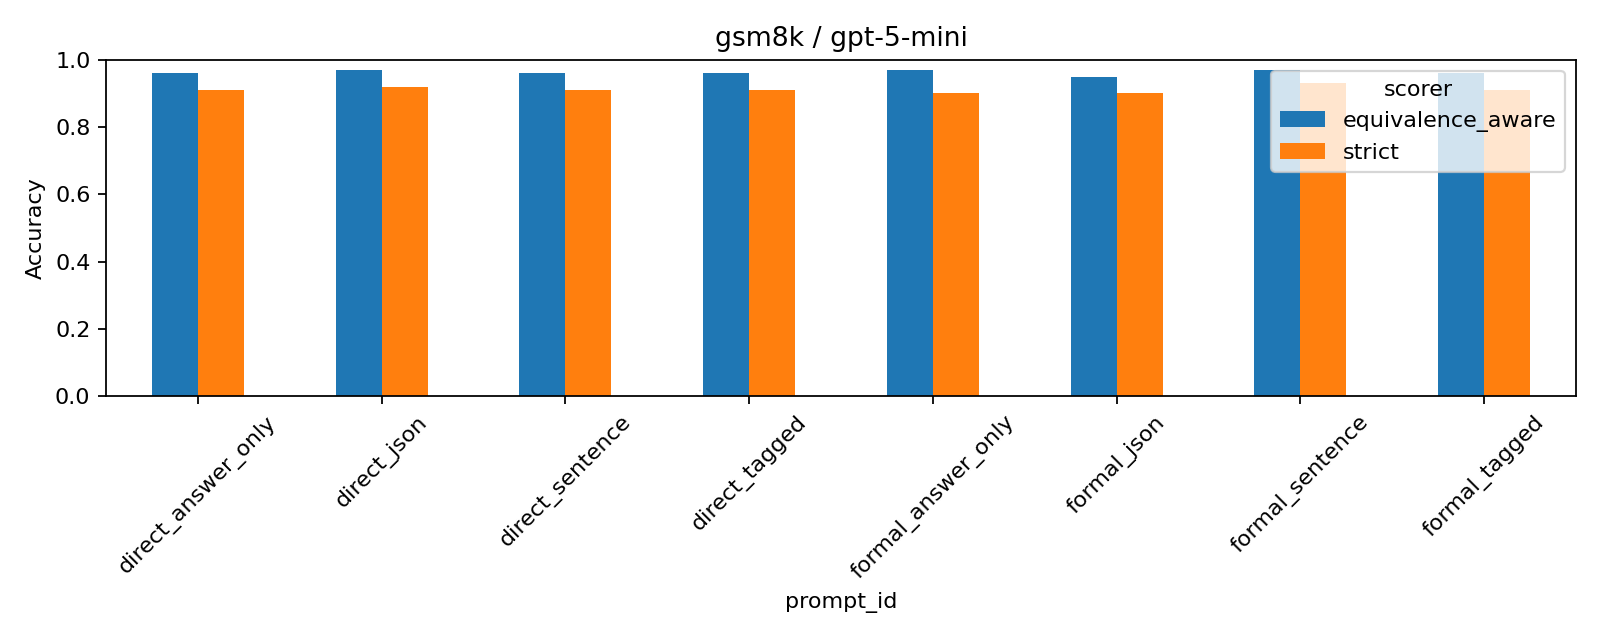
\includegraphics[width=\linewidth]{figures/accuracy_gsm8k_gpt-5-mini.png}

      \small \texttt{gpt-5-mini}
    \end{column}
    \begin{column}{0.5\linewidth}
      \centering
      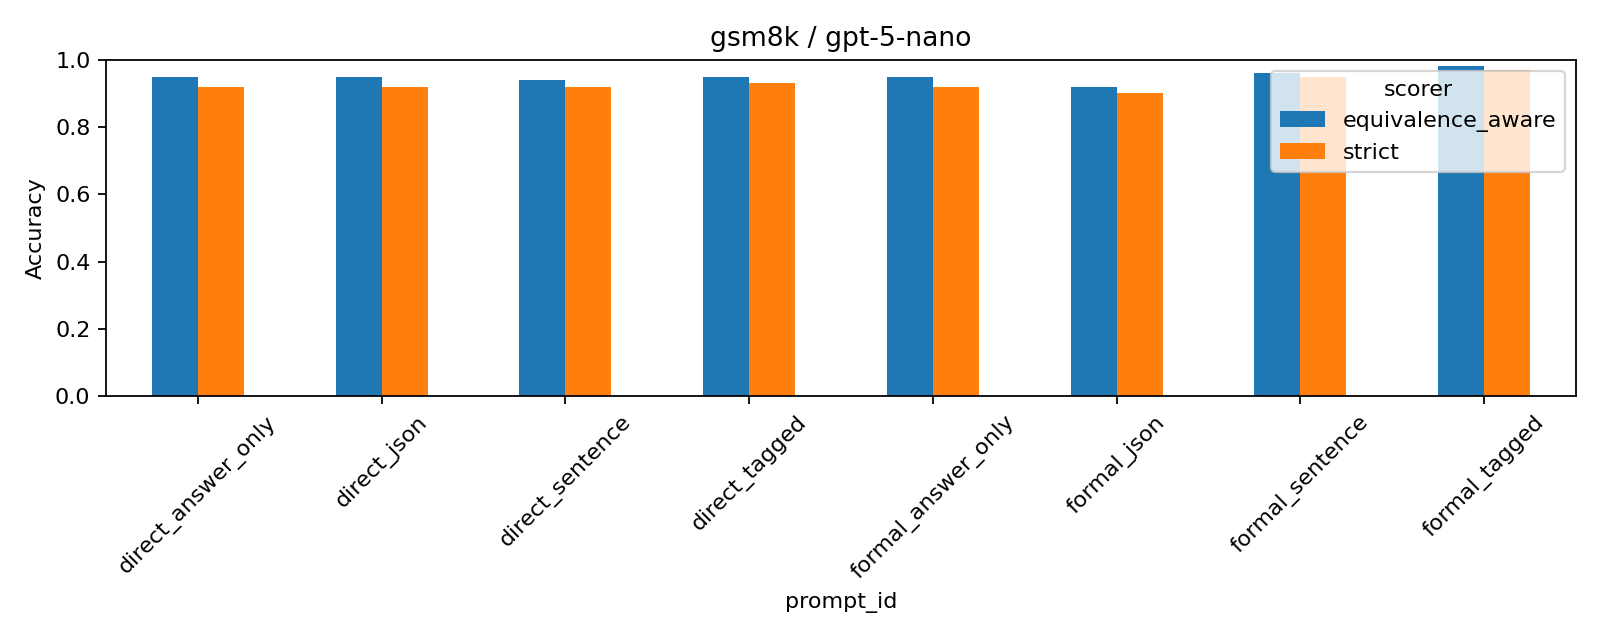
\includegraphics[width=\linewidth]{figures/accuracy_gsm8k_gpt-5-nano.png}

      \small \texttt{gpt-5-nano}
    \end{column}
  \end{columns}

  \vspace{0.8em}
  \begin{itemize}
    \item Equivalence-aware scoring recovers some strict-scoring misses.
    \item Recovery comes mostly from benign numeric formatting differences.
  \end{itemize}
\end{frame}

\begin{frame}{Prompt-Level Accuracy: TREC-6}
  \begin{columns}[T]
    \begin{column}{0.5\linewidth}
      \centering
      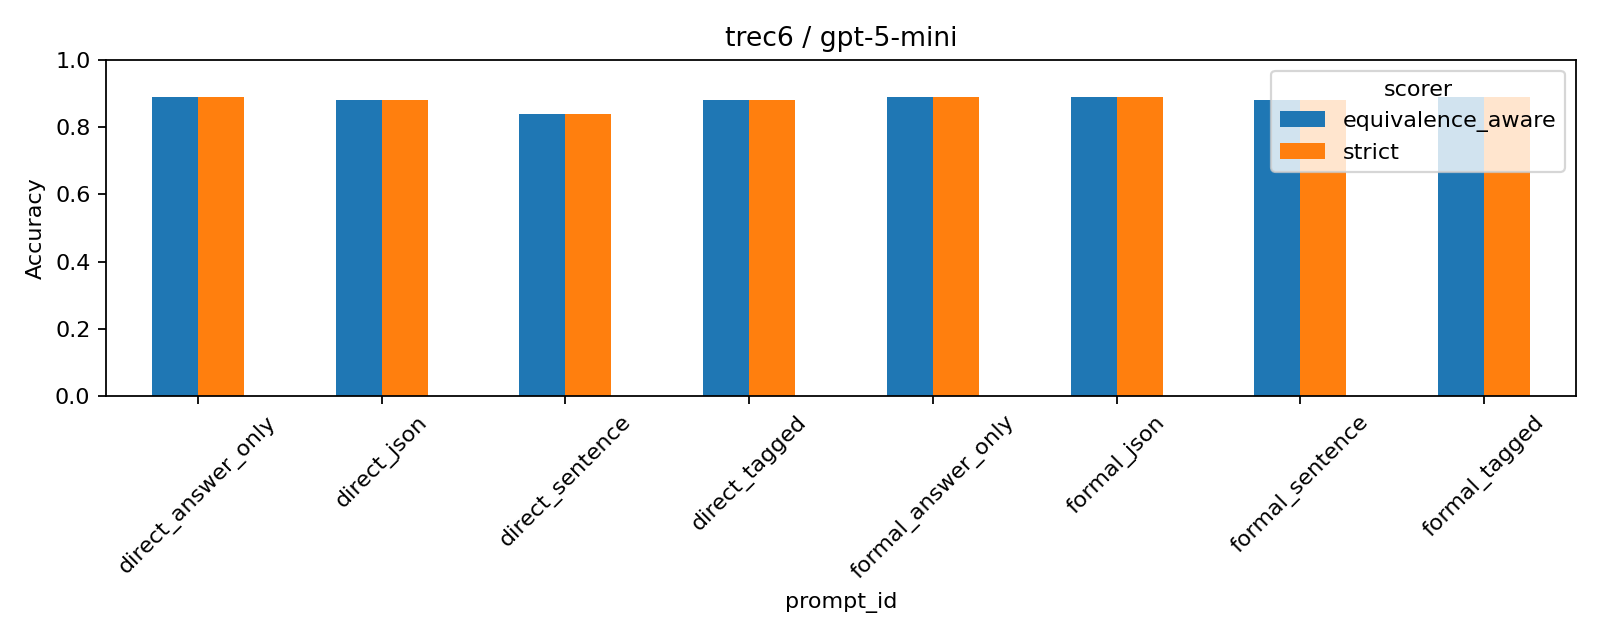
\includegraphics[width=\linewidth]{figures/accuracy_trec6_gpt-5-mini.png}

      \small \texttt{gpt-5-mini}
    \end{column}
    \begin{column}{0.5\linewidth}
      \centering
      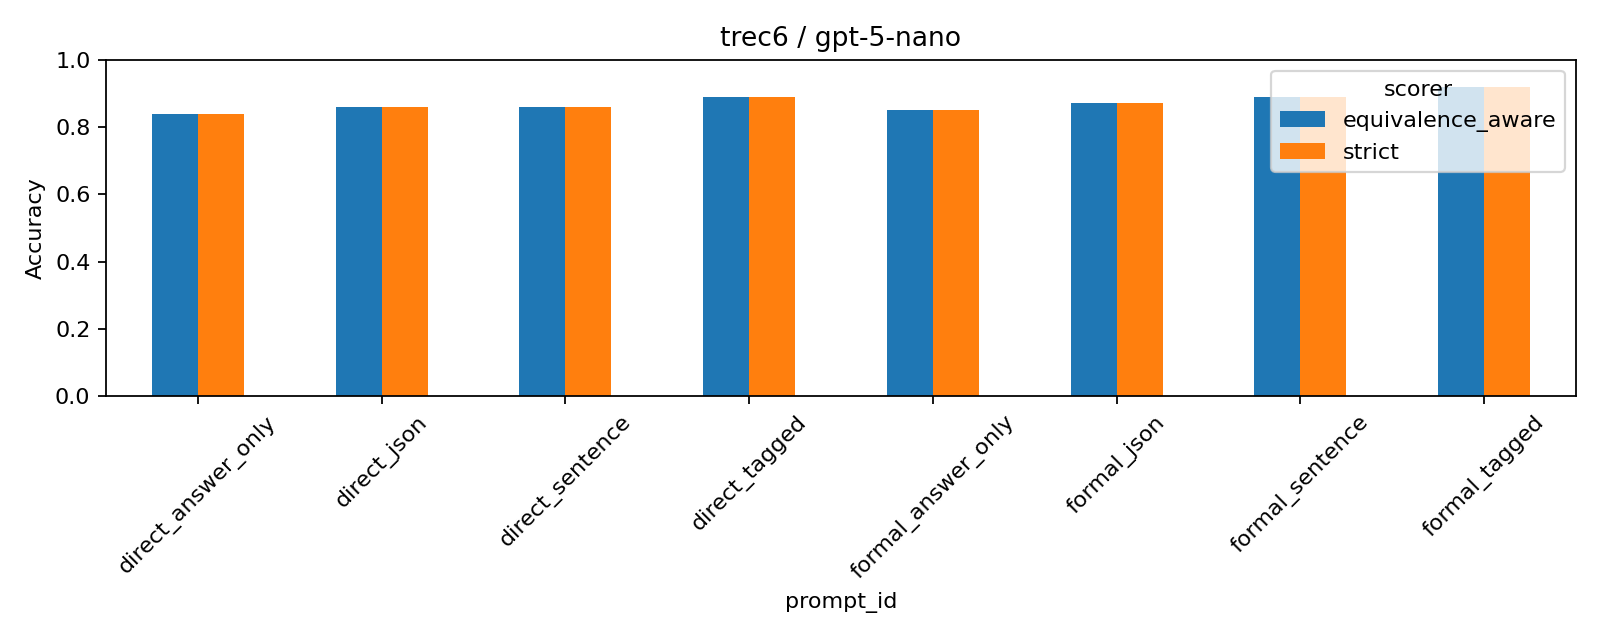
\includegraphics[width=\linewidth]{figures/accuracy_trec6_gpt-5-nano.png}

      \small \texttt{gpt-5-nano}
    \end{column}
  \end{columns}

  \vspace{0.8em}
  \begin{itemize}
    \item Strict and equivalence-aware bars overlap.
    \item The remaining errors are label errors, not formatting artifacts.
  \end{itemize}
\end{frame}

\begin{frame}{Error Analysis}
  \begin{columns}[T]
    \begin{column}{0.48\linewidth}
      \textbf{GSM8K}
      \smallgap
      \begin{itemize}
        \item wrong final numeric values
        \item correct values with harmless formatting differences
        \item examples: \texttt{5} vs. \texttt{5.00}, \texttt{5600} vs. \texttt{5,600}
      \end{itemize}
    \end{column}
    \begin{column}{0.48\linewidth}
      \textbf{TREC-6}
      \smallgap
      \begin{itemize}
        \item wrong category predictions
        \item common confusions: \texttt{ENTY} vs. \texttt{DESC}, \texttt{LOC} vs. \texttt{ENTY}
        \item little for equivalence-aware scoring to recover
      \end{itemize}
    \end{column}
  \end{columns}
\end{frame}

\begin{frame}{LLM-Judge Audit}
  \begin{itemize}
    \item Audited all outputs with \texttt{strict\_correct = false}.
    \item Judge model: \texttt{gpt-5.4}.
    \item Total judged records: 326.
  \end{itemize}

  \vspace{0.8em}
  \begin{table}
    \centering
    \begin{tabular}{lr}
      \toprule
      Outcome & Value \\
      \midrule
      Parse failures & 0 \\
      Agreement with deterministic scorer & 100\% \\
      Judge recovered rule misses & 0 \\
      Judge rejected rule recoveries & 0 \\
      \bottomrule
    \end{tabular}
  \end{table}

  \begin{block}{Interpretation}
    The audit supports that the deterministic equivalence-aware scorer is adequate for these structured tasks.
  \end{block}
\end{frame}

\begin{frame}{Limitations}
  \begin{itemize}
    \item Two tasks and two main models.
    \item One provider.
    \item 100 examples per task.
    \item One run per model/example/prompt condition.
    \item No human evaluation.
    \item Equivalence-aware scorer is task-specific.
  \end{itemize}

  \vspace{0.8em}
  \begin{block}{Interpretation caveat}
    Small differences of a few percentage points may include finite-sample noise. The result is best read as observed prompt-associated variation, not definitive statistical separation between every prompt template.
  \end{block}
\end{frame}

\begin{frame}{Takeaways}
  \begin{enumerate}
    \item Prompt choice changes measured accuracy even when task, examples, model, and scorer are fixed.
    \item Equivalence-aware scoring removes some formatting artifacts on GSM8K, but prompt sensitivity does not disappear.
    \item TREC-6 variation is driven by label prediction differences, not scoring artifacts.
    \item \texttt{gpt-5-nano} is more prompt-sensitive than \texttt{gpt-5-mini} despite similar average accuracy in some settings.
    \item Multi-prompt evaluation and careful scorer design both matter.
  \end{enumerate}
\end{frame}

\begin{frame}{One-Sentence Summary}
  \begin{block}{Final thesis}
    Modern LLM scores can move by several percentage points under semantically equivalent prompt and output-format changes; equivalence-aware scoring removes some formatting artifacts, but prompt sensitivity remains.
  \end{block}
\end{frame}

\end{document}

